\def\year{2018}\relax
%File: formatting-instruction.tex
\documentclass[letterpaper]{article} %DO NOT CHANGE THIS
\usepackage{aaai18}  %Required
\usepackage{times}  %Required
\usepackage{helvet}  %Required
\usepackage{courier}  %Required
\usepackage{url}  %Required
\usepackage{graphicx}  %Required
\frenchspacing  %Required
\setlength{\pdfpagewidth}{8.5in}  %Required
\setlength{\pdfpageheight}{11in}  %Required

\graphicspath{ {./images/} }
%PDF Info Is Required:
  \pdfinfo{
/Title (Heart Disease Classifier)
/Author (AAAI Press Staff)}
\setcounter{secnumdepth}{0}  
 \begin{document}
% The file aaai.sty is the style file for AAAI Press 
% proceedings, working notes, and technical reports.
%
\title{Heart Disease Classifier}
\author{Group 18: Zhong Yuyi, Zhang Junda, Mao Yancan, Li Denghao, Li Bo, Zhu Leyan\\
\begin{tabular}{c c c}
A0179956A & Zhong Yuyi & leader, logistic regression model for dataset 2 \\
A0178644R & Li Denghao & data processing, GBDT for dataset 1 and dataset 2, LSTM for dataset 3 \\
A0179822U & Li Bo & data processing, logistic regression model for dataset 1, naive Bayesian model for  dataset 2 \\
A0179892E & Zhang Junda & visualization and front-end implementation\\
A0179802X & Zhu Leyan & SVM for dataset 2  \\
A0179959X & Mao Yancan & data processing, GBDT, SVM, naive Bayesian model and neural network for dataset 1 \\
\end{tabular}
}
\maketitle
\begin{abstract}
Heart disease is one of the most serious health problems for people nowadays. To detect heart disease in a faster and more accurate way can help Singaporeans increase health standard. Based on the aforementioned consideration, we propose an application which is meant for analyzing and predicting the heart disease. To implement this application, we trained specific machine learning models on three different datasets. In overall, we tried five models including LTSM, GBDT, naive Bayesian, SVM and logistic regression, and picked GBDT for the first and second datasets and LSTM for the third dataset based on their better performance. Our application is believed to have good performance and reliability based on the experiments we have done so far, and thus might help Singaporeans to live a better life with respect to heart disease issue.
\end{abstract}

\section{Introduction}

Health is always the most concerned topic of people. Heart disease, in an academic expression cardiovascular disease, has been the most dangerous killer of human beings for long. A statistical data collected from more than 190 countries shows that every year 17.3 million deaths are related with heart disease, which remains the No. 1 global cause of death\footnote{\url{http://www.who.int/cardiovascular_diseases/en/}} \cite{WHO2016}. According to a study\footnote{\url{http://www.myheart.org.sg/article/about-the-heart-and-heart-disease/statistics/singapore/75}} \cite{singapore2016}, Singaporeans suffer heart failure about 10 years earlier than Americans and Europeans, and nearly 1 in 3 Singaporeans are dying from heart disease. In order to increase the average health standard for Singaporeans, one of the best way is to examine people's heart condition early and find the pathogeny accurately.

In this report we are going to introduce an application which can help analyzing and predicting the heart disease in two specific aspects: Cardiac Arrhythmia and Cardiovascular diseases. We first collect the basic information about patients such as age, gender, resting blood pressure and so on give a general diagnosis (first step). Then we will further examine the heart rhythm (second step) and heart sounds (third step) of patients. The diagnosis of heart rhythm is classified into 13 classes and diagnosis of heart sounds is classified into 3 classes. Based on these 3 steps and detailed classifications, doctors can have more confidence to give a accurate analysis result, which also help curing patients correctly and effectively.
 
To achieve this goal we used 3 datasets, one dataset for each step. The first dataset dated from 1988 and consists of four databases: Cleveland, Hungary, Switzerland, and Long Beach VA\footnote{UCI Heart Disease Dataset. \url{https://archive.ics.uci.edu/ml/datasets/Heart+Disease}} \cite{1988heart}. Each database provides 76 attributes, including the predicted attribute. The second dataset are based on the Electrocardiogram (ECG) readings and other attributes\footnote{UCI Arrhythmia Dataset. \url{https://archive.ics.uci.edu/ml/datasets/Arrhythmia}} \cite{guvenir1998arrhythmia}. There are 279 attributes in total and grouped into 5 blocks: features concerning biographical characteristics, features concerning average wave durations of each interval, features concerning vector angles of each wave, features concerning widths of each wave and features concerning amplitudes of each wave. The third dataset is wave files gathered from two sources\footnote{Heart Sound Dataset. \url{https://www.kaggle.com/kinguistics/heartbeat-sounds/data}} \cite{king2017heart}: (A) from the general public via the iStethoscope Pro iPhone app, provided in Dataset A, and (B) from a clinic trial in hospitals using the digital stethoscope DigiScope, provided in Dataset B. Some of the attributes value are missing in these three datasets, so we do some pre-handling process with each dataset. After comparing different machine learning models and adjusting parameters related, we use Gradient Boosting Decision Tree (GBDT) for the first and second datasets, and Long Short-Term Memory (LSTM) for the third dataset because of their good performance.

Our work is available at GitHub\footnote{\url{https://github.com/yancanmao/ML-project}}.

\section{Related Works}

Recently, lots of efforts have been made to machine intelligence aided diagnosis of heart disease. Related researches mostly focus on analysis of one or two dimensional bio-signals. 

One dimensional signal includes heartbeat sound and electrocardiogram. Heart sound can help with diagnosis mainly through detection of murmur heart sound and extra systole, which imply certain kinds of cardiac disease. Though features extraction methods for detection abnormal heart sound had been researched for decades, modern method outperforms traditional feature extraction \cite{chen2017s1}. Electrocardiogram (ECG) is also an important information source for diagnosis. Researchers from Stanford University made contribution to arrhythmia detection and classification based on a CNN model for ECG signals \cite{rajpurkar2017cardiologist}. These signals can offer limited but straight forward clues for heart abnormalities. 

As for bio-images, MRI data were first studied. FCN was used for cardiac MRI segmentation back in 2016 \cite{tran2016fully}. This kind of tasks then were heavily discussed. Researchers at University of California successfully implemented a fast and accurate view classification of echocardiograms, one of the most essential examinations to cardiology using deep learning \cite{madani2018fast}. However, MRI segmentation or echocardiograms view classification are only preprocessing for images, which in fact doesn’t touch the core of heart disease diagnosis. Direct diagnosis via machine learning still has a long way to go. Images of organ other than heart are also reported in works. Researchers from Google and Verily constructed a deep learning model for prediction of age, gender, smoking status, systolic blood pressure and major adverse cardiac events via retinal images \cite{poplin2018prediction}. These works are based on huge image data which are not accessible to most researchers thus machine diagnosis via images is still limited and needs deeper studies.

\section{Method}

\subsection{Model Description}

\subsubsection{GBDT}

Gradient boosting is a machine learning technique for regression, classification and sorting tasks. It belongs to boosting algorithm family, which can enhance a weak learner to a strong learner. Boosting algorithms are based on the idea that it's better to get a result by synthesizing many experts' judgements than getting it from only one of them. Gradient boosting, same as other boosting algorithms, constructs the final prediction model with an ensemble of many weak learners, usually decision tree. This is what we call Gradient Boosting Decision Tree.

Boosting is one of the major methods of ensemble learning \cite{li2016gentle}. It constructs model using a stage-wise iterative method. The weak learner constructed at every step of iteration is designed to make up for the deficiency of the existing model. Gradient boosting does it by construct a learner that reduces the loss along the steepest gradient in each step. Gradient boosting has an enormous scope of application since it is capable of processing all kinds of learning tasks by setting different loss functions. It can resist noise in training data effectively as well.

Gradient boosting algorithm tends to use decision tree because this algorithm is easy to understand and has strong interpretability and rapid forecasting speed. Also, decision tree algorithm can process data with missing fields well and do not need to consider interdependence between features.

According to above, Gradient Boosting Decision Tree is one of the best, state-of-the-art machine learning algorithms. Therefore, we choose it for our first two datasets.

\subsubsection{LSTM}

Long Short-Term Memory is a variant of recurrent neural network, which uses special units that can maintain information in memory for long periods of time in addition to standard units, which allows for a better control over the gradient flow and enable better preservation of ``long-range dependencies''\footnote{A Beginner's Guide to Recurrent Networks and LSTMs. \url{https://deeplearning4j.org/lstm}}. The key point for implementing LSTM is to figure out what to forget, save and ignore as a memory cell. Since LSTM is a state-of-art deep learning method and has been widely used on different topics with great performance, we picked this model to see how it works for our application.

Basically, we are able to observe two types of abnormalities in a piece of heart sound: murmur, which indicates the blood reverse flow caused by mitral insufficiency, and extra systole, which indicates myocardial injury. These two kinds of abnormalities are independent, so in our work, we extract the starting part of Fourier transform power (frequency lower than 470Hz) and a binary sequence marking the existence of heart beat pulse in 0.075s time interval (about the width of a pulse) as sequential features for murmur heart sound and extra systole respectively. 

We built two two-layer LSTM models. The first is aimed to classify murmur heart sound, where the input is the starting part of Fourier transform power and the input length of hidden layer (also the output length of input layer) is 8, and the output length of hidden layer (also the input length of dense output layer) is 4. The second is aimed to classify extra systole, where the input is the binary sequence marking the existence of heart beat pulse and the input length of hidden layer is 8, and the output length of hidden layer is 8. 

\subsection{Application Display}

We design a web application with Bottle\footnote{Bottle: Python Web Framework. \url{http://bottlepy.org}} as the back-end framework of our application and Bootstrap\footnote{Bootstrap: an open source toolkit for developing with HTML, CSS, and JS. \url{https://getbootstrap.com/}} as the front-end library. We provide two functions for our users:

\begin{itemize}
\item Predict the risk of heart disease based on biographical information
\item Predict murmur heart sound or extra systole risk based on heart sound wave file
\end{itemize}

For the first function, users have to fill 14 attributes such as age, sex and so on to get better accurate prediction. We'll return a result based on the ranking for users to show if they have a risk of heart disease or not. The user interface is showed in Figure \ref{fig:dataset-1-ui}.

\begin{figure}[!htbp]
\centering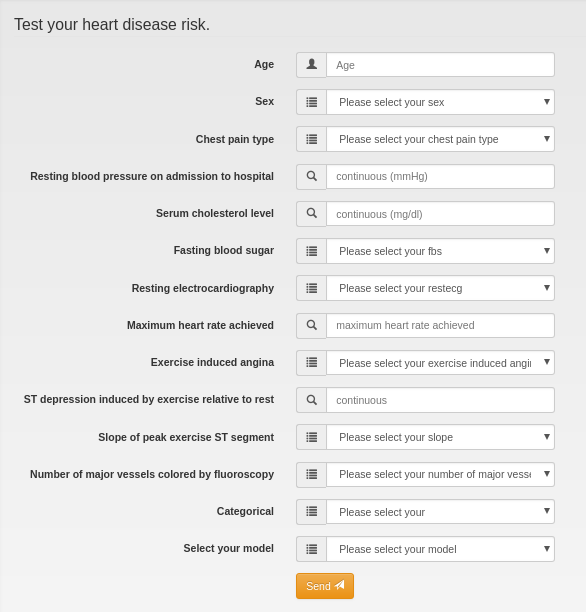
\includegraphics[width=0.45\textwidth]{dataset-1-ui}
\caption{User interface for the first function}
\label{fig:dataset-1-ui}
\end{figure}

For the second function, users have to upload their heart sound wave files recorded from their mobile to predict the risk of two kinds of abnormal heart sound, murmur and extra systole. We use models trained on dataset 3 to predict in back-end. We'll get two probabilities of murmur and extra systole respectively. If the probabilities are too high, then we'll tell users they may have the risk. The user interface is showed in Figure \ref{fig:dataset-3-ui}.

\begin{figure}[!htbp]
\centering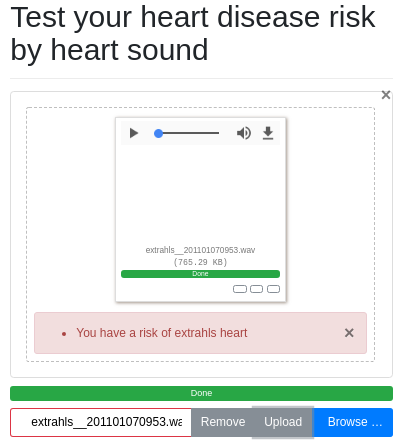
\includegraphics[width=0.45\textwidth]{dataset-3-ui}
\caption{User interface for the second function}
\label{fig:dataset-3-ui}
\end{figure}

\section{Experiment}

\subsection{Experiment Setup}

We have released our project on Github, and to see more details about our application, you can setup an experiment by yourself. Our project is running as a website. To setup the service, first ensure you have installed Anaconda3\footnote{\url{https://www.anaconda.com/download/}} and python library LightGBM\footnote{\url{http://lightgbm.readthedocs.io/en/latest/}}. Secondly, you should install front-end framework package Bootstrap and back-end framework package Bottle. Then you can run the service in our repository.

\subsection{Model Evaluation and Comparison}

As explained above, our heart disease testing based on three data sources: biographical information, ECG and heart sound.

There are many missing attribute values in biographical dataset we derived from UCI. In addition, the Cleveland data set became corrupted after the loss of a computing node, and the surviving data set contains only 14 attributes per instance (shown in Figure \ref{fig:dataset-1}). Therefore, we constructed a 14 attributes dataset with 920 instances, and the last row (``num'') is the attribute to be predicted. In these instances, some of them also have unobserved attributes. For all of unobserved attributes, we replaced them to a certain negative number never appeared in the samples which means unobserved, and we divide the whole dataset into training data and test data with a proportion of 4:1. All models compared below for dataset 1 used this pre-processed dataset.

\begin{figure}[!htbp]
\centering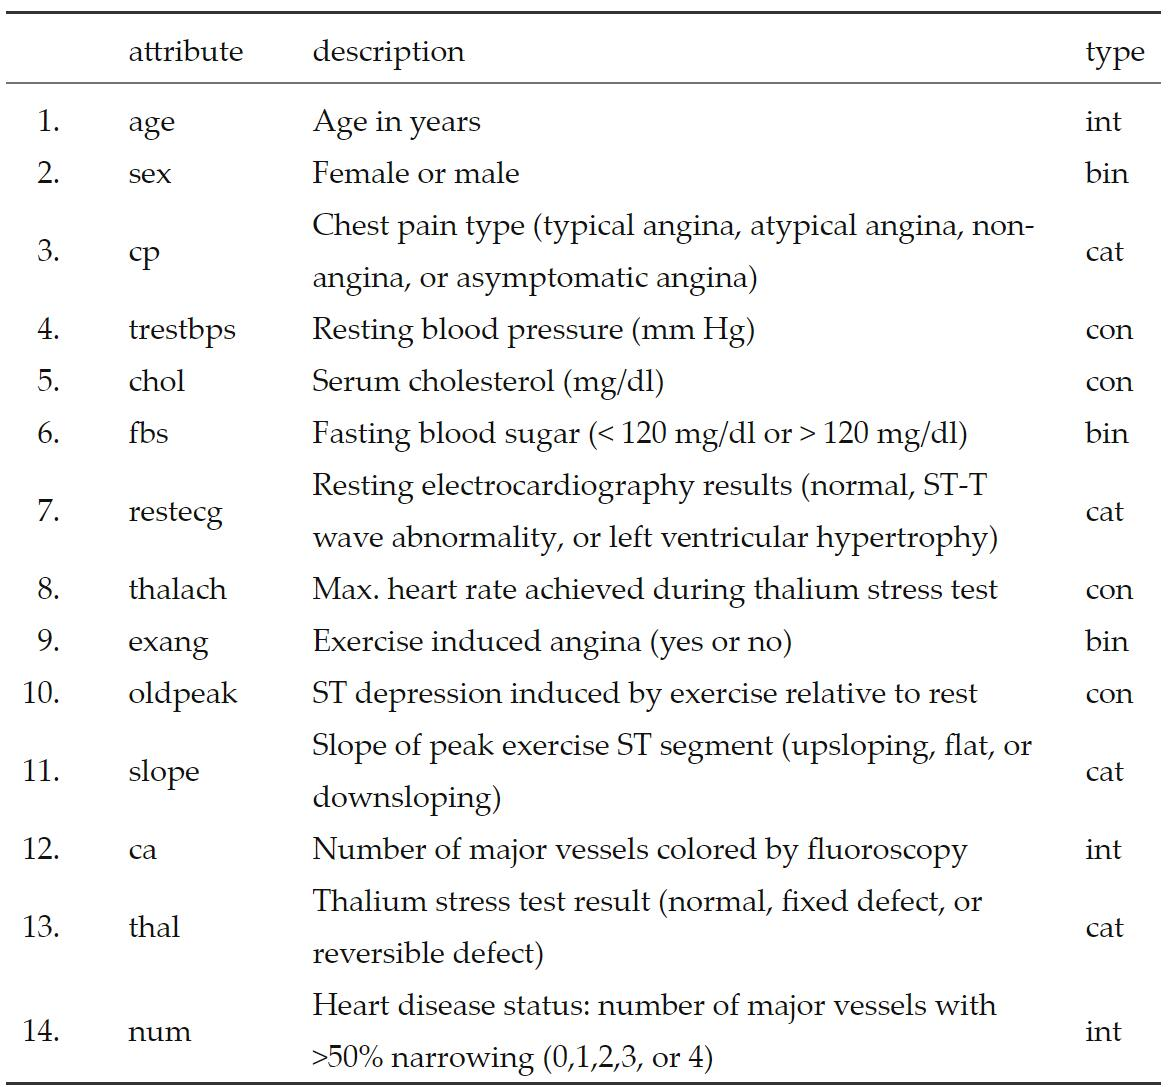
\includegraphics[width=0.4\textwidth]{dataset-1}
\caption{Biographical attributes}
\label{fig:dataset-1}
\end{figure}

This biographical dataset was used at the first step of our application, it provides basic information. Because its attributes are limited and could be commonly measured, our application uses this dataset to train a general classifier. We have trained it with five models: GBDT, naive Bayes, SVM, neural network and logistic regression. 

We regard biographical information as a vector indicating a sample in the sample space. And for the ECG data, we use the method introduced by Guvenir et al. in \cite{guvenir1997supervised} to extract a 275 dimensional feature for each sample.  For this classification task, we tested four binary classification models: logistic regression, naive Bayes, SVM and GBDT. 

Each member of our group developed one or more of models for these datasets. After comparing the accuracy between these models with each model's best performance on this dataset (see Figure \ref{fig:dataset-1-comparison}), we found that GBDT had highest and most stable accuracy about 89.57\%. As a result, we chose LightGBM as our final training library. LightGBM is an efficient, low memory usage library. Additionally, it can be used for almost all regression problems, and our classifier is exactly one of them. The performance of the four models on dataset 1 and dataset 2 are shown at Figure \ref{fig:dataset-1-comparison}:

\begin{figure}[!htbp]
\centering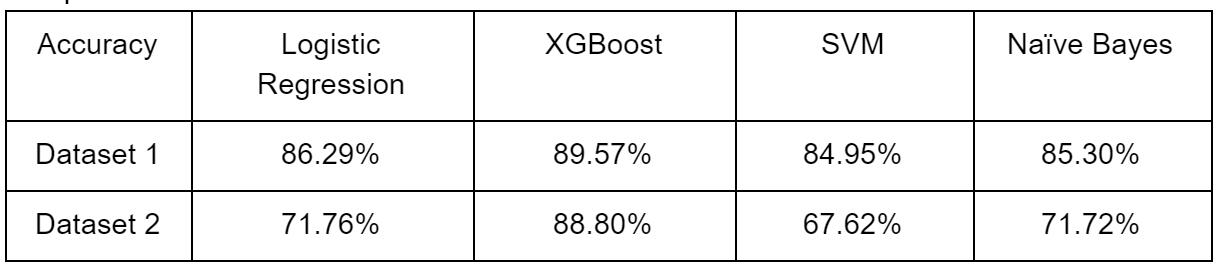
\includegraphics[width=0.45\textwidth]{dataset-1-comparison}
\caption{The result of different binary classification models}
\label{fig:dataset-1-comparison}
\end{figure}

The information we can derive the heart sound is limited as it is prone to be contaminated by environment noise. We trained the murmur detection model and the extra systole detection model for 200 and 100 epochs respectively with both learning rate equal to 0.001. The evaluation of the two LSTM models are shown below:

\begin{figure}[!htbp]
\centering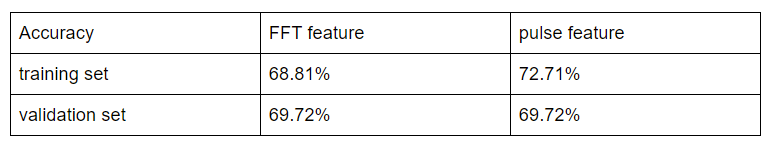
\includegraphics[width=0.45\textwidth]{dataset-3-comparison}
\caption{Evaluation of LSTM model}
\label{fig:dataset-3-comparison}
\end{figure}

\subsection{Optimization method}

We used grid search for GBDT parameters to optimize the performance. We used Sklearn to invoke Logistic Regression, SVM and Naive Bayes models. Logistic regression has the second best accuracy on both dataset 1 and dataset 2. The optimization method for all of these three method is to select columns to make the cross validation be best, which aims to avoid overfitting. Excepting for select columns method, we also have different methods for different models.

\subsubsection{GBDT Optimization}

At the beginning of the training, when using default parameters of GBDT model, we got an accuracy 82.83\% which is low. Therefore, we tried to improve the accuracy of model's performance. On the one hand, we eliminated some least important attributes in this model by using Pandas (the importance of every attributes using in LightGBM are shown at Figure \ref{fig:dataset-1-impor}):

\begin{figure}[!htbp]
\centering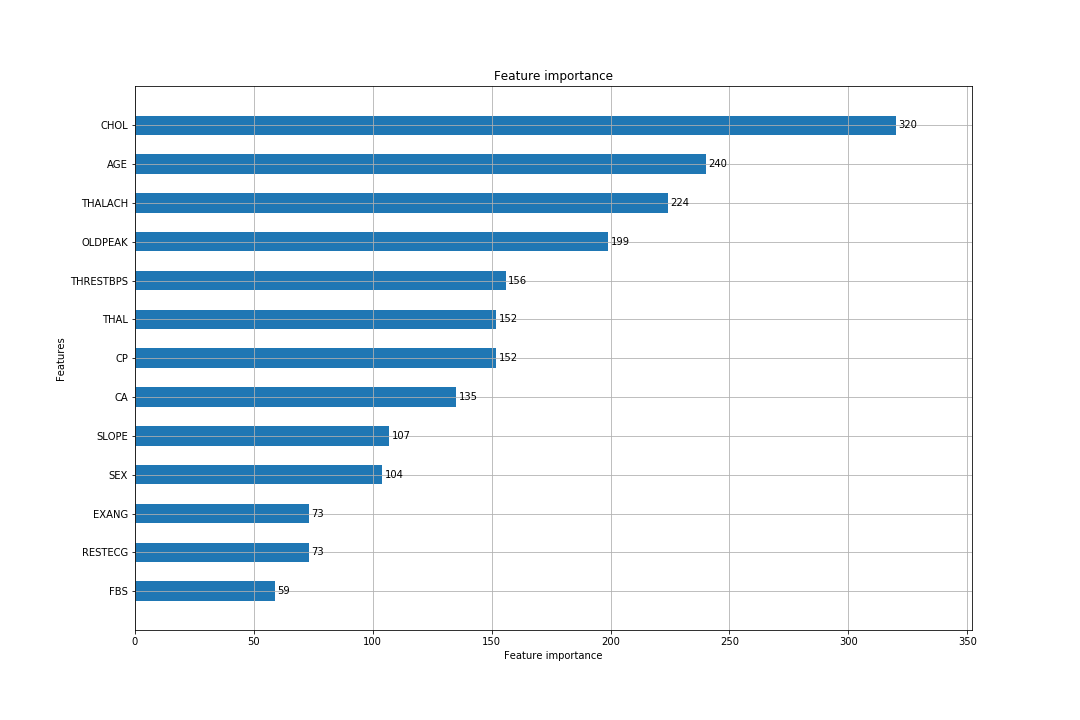
\includegraphics[width=0.45\textwidth]{dataset-1-impor}
\caption{Importance of attributes in LightGBM}
\label{fig:dataset-1-impor}
\end{figure}

we attempted to eliminate FBS and RESTECG, but the accuracy dropped, so we didn't modify attributes using this model. On the other hand, we modified LightGBM model's attributes by using grid search method which continuously modifies parameters of model's including number of leaves, minimum data in a leaf, learning rate and so on, and then finds the parameters result with best accuracy. Finally, we got a optimal result with accuracy 89.57\%.

\subsubsection{Logistic Regression Optimization}

In Logistic Regression, things we should do are to analyze the fit coefficient, and drop columns with negative fit coefficient. In this way, our training time shortened a lot \cite{brownlee2016logistic}. We also tried some parameters Sklearn provides, we modified penalty parameter to 'l1' to avoid overfitting, and we tried C parameter to modify inverse of regularization strength\footnote{Logistic Regression in sklearn. \url{http://scikit-learn.org/stable/modules/linear_model.html#logistic-regression}}.

\subsubsection{SVM Optimization}

For SVM we tried 4 different kernel functions\footnote{SVM in sklearn. \url{http://scikit-learn.org/stable/modules/svm.html}}.
\begin{itemize}
\item Linear Kernel Function:$K(x_i,x_j)=x_i^Tx_j$.
\item Polynomial Kernel Function: $K(x_i,x_j)=(\gamma x_i^T x_j+r)^d,d>1$.
\item RBF Kernel Function: $K(x_i,x_j)=exp(-\gamma||x_i-x_j||^2),\gamma>0$.
\item Sigmod Kernel Function: $K(x_i,x_j)=tanh(\gamma x_i^T x_j+r), \gamma>0,r<0$.
\end{itemize}

After comparing different kernel functions, the linear one with the penalty parameter c = 2 gives best expected accuracy 67.62\%.

\subsubsection{Naive Bayes Optimization}

For Naive Bayes, three different algorithms of it are provided in scikit-learn\footnote{Naive Bayes in sklearn. \url{http://scikit-learn.org/stable/modules/naive_bayes.html}}.

\begin{itemize}
\item GaussianNB: The prior is Gaussian distribution. It is commonly used when the distributions of most sample features are continuous values.$P(X_j|Y=C_k) = \frac{1}{\sqrt{2 \pi \sigma_k^2}}exp(\frac{(x_j-u_k)^2}{2\sigma^2})$.
\item MultinomialNB: The prior is Multinomial distribution. It is suitable when the distributions of most sample features are multivariate discrete values.$P(X_j|Y=C_k)=\frac{x_j+\lambda}{M_k+n\lambda}$
\item BernoulliNB: The prior is Bernoulli distribution. We choose this when the distributions of sample features are binary discrete values or very sparse multivariate discrete values.$P(X_j=x_j|Y=C_k)=P(j|Y=C_k)x_j+(1-P(j|Y=C_k))(1-x_j)$
\end{itemize}

After comparing the performance of these three distributions, we chose GaussianNB for dataset 1 and BernoulliNB for dataset 2.

\section{Conclusion}

We implemented an application meant for heart disease detecting, which used three different aspects including overall healthy condition, cardiac arrhythmia and heartbeat sounds to diagnose the final result step by step. By the end, we obtained relatively reliable performance and provided a platform for other users. It should be noted that we tried several models on three datasets and picked up the optimal model as the final model for our application. Through this project, we learned how to do demand analysis, performance evaluation and also fine tuning skills, which help us to understand machine learning further.

\newpage
%\section{References}
\bibliographystyle{aaai}
\bibliography{report.bib}

\end{document}
